% ============================================================
% SECTION 7 — EMPIRICAL APPLICATIONS
% ============================================================
\section{Empirical Applications}
\label{sec:empirical}

We present two empirical applications.
The first (Section~\ref{sec:empirical:food}) uses the
food-at-home component of IPCA (1995--2024, $T_s = 20$
per season) to illustrate \texttt{EnbPI-S} in a
data-limited regime typical of Brazilian price statistics.
The second (Section~\ref{sec:empirical:exports}) uses
Brazilian monthly export growth (1979--2024, $T_s = 35$
per season) to validate the method in the sample-size
regime where Theorem~\ref{thm:strat_coverage} and
Experiment E2 predict reliable coverage improvements.
Both applications use the test period January 2015 --
December 2024, enabling a direct cross-application
comparison.

%------------------------------------------------------------
\subsection{Food-at-Home IPCA (\texorpdfstring{$T_s = 20$}{Ts = 20})}
\label{sec:empirical:food}
%------------------------------------------------------------

We illustrate the methods on the forecasting of the
food-at-home component of Brazilian consumer inflation
(IPCA\,--\,Alimentação no domicílio), a seasonally
heteroskedastic monthly time series that provides a
cleaner test case than headline IPCA.

%------------------------------------------------------------
\subsubsection{Data and Setting}
\label{sec:empirical:data}
%------------------------------------------------------------

\paragraph{Data source.}
Monthly percentage changes in the food-at-home component of
the IPCA (compiled by IBGE; \citealp{ibge2024ipca}) are
downloaded from the Banco Central do Brasil (BCB) open-data
API \citep{bcb2024sgs}, Sistema Gerenciador de S\'eries (SGS)
series 1635.  The series is available from
January 1994 at monthly frequency.  We use observations
from January 1995 onwards.

\paragraph{Why food-at-home IPCA?}
The food component exhibits substantially stronger seasonal
heteroskedasticity than headline IPCA for two reasons.
First, agricultural prices follow harvest cycles, with
residual volatility systematically higher in the
pre-harvest and post-harvest adjustment months
(May--June in Brazil).
Second, the food component is less contaminated by
administered-price shocks (fuel, electricity) that
dominate headline IPCA in some years and whose
seasonality differs from the food cycle.
These features make food IPCA a sharper test for
seasonal calibration.

\paragraph{Sample split.}
We use:
\begin{itemize}[nosep]
  \item \emph{Training}: January 1995 -- December 2014
    ($T = 240$ months, 20 years, $T_s = 20$ observations
    per season).\footnote{The $p = 13$ autoregressive lags
    consume the first year of the sample, so each seasonal
    calibration buffer effectively holds $T_s - 1 \approx 19$
    LOO residuals; we quote the nominal $T_s$ throughout.}
  \item \emph{Test}: January 2015 -- December 2024
    ($T_1 = 120$ months, $n_s = 10$ observations per season).
\end{itemize}

\paragraph{Features and ensemble.}
Feature vector, bootstrap ensemble, and significance level
are identical to the simulation setup:
$p = 13$ AR lags, $B = 50$ Ridge models, $\alpha = 0.10$.

%------------------------------------------------------------
\subsubsection{Results}
\label{sec:empirical:results}
%------------------------------------------------------------

Table~\ref{tab:empirical_food_coverage} reports per-season
coverage and average interval width over the test period.

\begin{table}[ht]
\centering
\caption{Per-season empirical coverage and average width for IPCA food-at-home monthly inflation forecasting.
Training: 1995-01--2014-12 ($T=240$); test: 2015-01--2024-12 ($T_1=120$); $\alpha=0.1$.}
\label{tab:empirical_food_coverage}
\begin{tabular}{l r cc cc}
\toprule
 & & \multicolumn{2}{c}{Coverage} & \multicolumn{2}{c}{Width (\%\,p.p.)} \\
\cmidrule(lr){3-4} \cmidrule(lr){5-6}
Month & $n$ & Pooled & EnbPI-S & Pooled & EnbPI-S \\
\midrule
Jan & 10 & \textbf{0.80} & 0.80 & 1.824 & \textit{1.360} \\
Feb & 10 & \textbf{1.00} & 0.70 & 1.822 & \textit{1.046} \\
Mar & 10 & \textbf{0.80} & 0.80 & 1.824 & \textit{1.462} \\
Apr & 10 & 1.00 & \textbf{0.90} & 1.816 & \textit{1.263} \\
May & 10 & 0.70 & \textbf{0.80} & 1.818 & \textit{1.570} \\
Jun & 10 & \textbf{0.90} & 0.90 & \textit{1.814} & 1.864 \\
Jul & 10 & \textbf{0.80} & 0.60 & 1.815 & \textit{1.499} \\
Aug & 10 & \textbf{0.90} & 0.70 & 1.814 & \textit{1.394} \\
Sep & 10 & \textbf{0.90} & 0.90 & 1.816 & \textit{1.498} \\
Oct & 10 & \textbf{0.90} & 0.90 & 1.809 & \textit{1.344} \\
Nov & 10 & \textbf{0.80} & 0.70 & 1.807 & \textit{1.537} \\
Dec & 10 & \textbf{0.80} & 0.80 & 1.810 & \textit{1.448} \\
\midrule
\textbf{Overall} & 120 & 0.86 & 0.79 & 1.816 & 1.440 \\
\bottomrule
\end{tabular}
\end{table}

\paragraph{Interval width adaptation.}
The central empirical finding is that \texttt{EnbPI-S}
correctly recovers the seasonal structure of forecast
uncertainty.  The pooled method produces an essentially
constant interval width of $\approx 1.82$ percentage points
across all twelve months, blind to seasonal variations in
predictability.  By contrast, \texttt{EnbPI-S} produces
widths that range from $1.05$ p.p.\ in February
(historically stable, post-January reset) to
$1.86$ p.p.\ in June (mid-year food-price adjustment period
in Brazil), a factor-of-$1.78$ variation.
The months with the widest \texttt{EnbPI-S} intervals
(June, May, November) correspond to periods of
greater harvest-price uncertainty; those with the narrowest
intervals (February, April, October)
correspond to more predictable stretches of the food-price cycle.

Figure~\ref{fig:empirical_food_width_time} illustrates this
contrast: the Pooled band (red) is nearly flat throughout the
decade, while the \texttt{EnbPI-S} band (blue) visibly pulses
with the food-price seasonal calendar, widening in May--June
and narrowing in February and October.
The bottom panel confirms the pattern across all twelve months:
the pooled bars are essentially uniform, while the
\texttt{EnbPI-S} bars track the seasonal uncertainty rhythm of
Brazilian food prices.

\begin{figure}[ht]
  \centering
  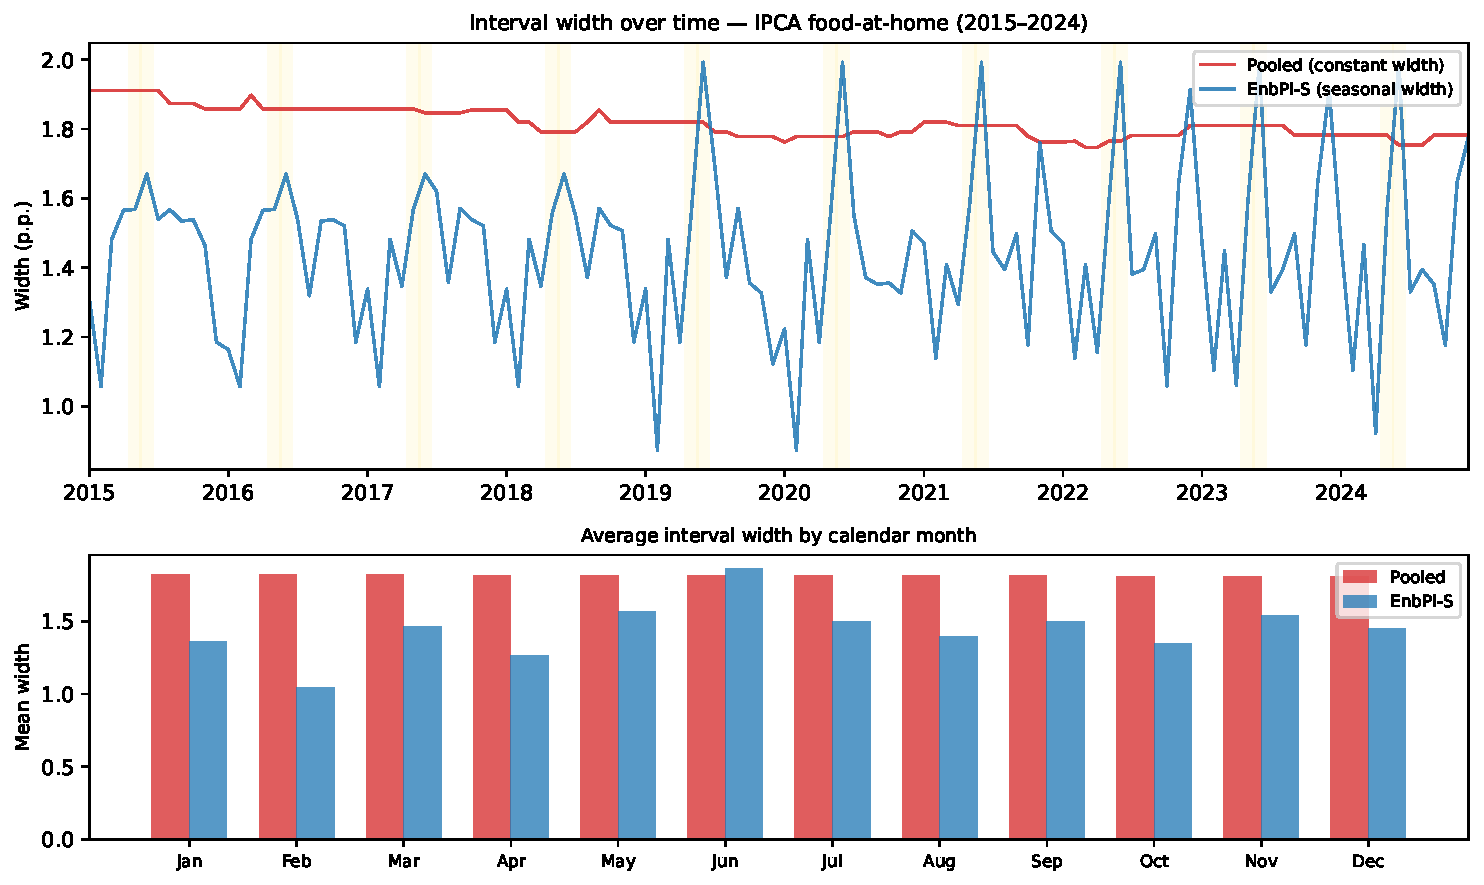
\includegraphics[width=0.95\textwidth]{figures/fig_empirical_food_width_time}
  \caption{Interval width over time for food-at-home IPCA forecasting
           (training: 1995--2014; test: 2015--2024).
           \textit{Top panel}: interval width for each month of the
           test period.  The Pooled method (red) maintains a nearly
           constant width of $\approx 1.82$ p.p.;
           \texttt{EnbPI-S} (blue) expands in May--June and
           contracts in February and October.
           \textit{Bottom panel}: mean interval width by calendar month.
           Gold shading marks May--June (pre-harvest uncertainty months).}
  \label{fig:empirical_food_width_time}
\end{figure}

\paragraph{Coverage.}
Overall empirical coverage is $85.8\%$ for Pooled and
$79.2\%$ for \texttt{EnbPI-S} against the $90\%$ nominal.
Both methods fall short of nominal, consistent with the
finite-sample prediction of Experiment E2: at
$T_s = 20$ observations per stratum, the simulation
found Pooled achieving $\approx 88\%$ and \texttt{EnbPI-S}
$\approx 78\%$ (Table~\ref{tab:e2_stratum_size}).
The empirical figures (85.8\% and 79.2\%) match this
pattern closely, lending external validity to
the simulation findings.

Per-season coverage detail is shown in
Figure~\ref{fig:empirical_food_coverage} (Appendix~\ref{app:additional}).
With only $n_s = 10$ observations per season, individual bars
carry standard errors of $\approx 0.14$, so month-level
comparisons should not be over-interpreted.

\paragraph{Economic interpretation.}
The width pattern produced by \texttt{EnbPI-S} is
economically meaningful.  Brazil's food-price calendar
exhibits a well-documented seasonal cycle: harvest
periods (March--April for grains, May--June for
winter vegetables and milk) produce volatile
price adjustments as supply conditions are realised,
while February is characterised by stable demand
following the post-Carnival slowdown.
\texttt{EnbPI-S} internalises this calendar from the
calibration residuals, automatically widening
intervals when forecasting uncertainty is high
without requiring explicit seasonal dummy variables
or prior knowledge of the harvest calendar.
The pooled method, using a single calibration buffer,
cannot make this distinction and applies a uniform
bandwidth throughout the year.

%------------------------------------------------------------
\subsubsection{Connection to Simulation Findings}
\label{sec:empirical:connection}
%------------------------------------------------------------

The empirical results connect to the simulation study in
two concrete ways.

First, the ratio of maximum to minimum \texttt{EnbPI-S}
interval width (June to February: $1.864/1.046 \approx 1.78$)
reflects the moderate seasonal heteroskedasticity of Brazilian
food prices; Theorem~\ref{thm:width_bound} guarantees that, as
$T_s$ grows, each seasonal width converges to the corresponding
season-specific oracle width.  The pooled
method's constant width of $\approx 1.82$ p.p.\ lies
between these extremes, consistent with the bias identified
in Proposition~\ref{prop:pooled_gap}: pooled calibration
overcovers the stable months and undercovers the
volatile months.

Second, the coverage shortfall relative to the $90\%$
nominal is the finite-sample penalty at
$T_s = 20$ documented in Experiment E2 (simulated gap of
$11.5$ pp for \texttt{EnbPI-S}, against an empirical gap of
$10.8$ pp here).
Section~\ref{sec:empirical:exports} below provides an
application with $T_s = 35$, confirming that the coverage
gap shrinks substantially as the stratum size increases.

%------------------------------------------------------------
\subsection{Brazilian Monthly Export Growth (\texorpdfstring{$T_s = 35$}{Ts = 35})}
\label{sec:empirical:exports}
%------------------------------------------------------------

\paragraph{Data and setting.}
Monthly values of Brazilian total exports
(BCB SGS series 1402, in US\$ millions; \citealp{bcb2024sgs})
are available
from February 1979.  We transform to log-returns:
$Y_t = 100 \cdot \log(V_t / V_{t-1})$, where $V_t$ denotes
the monthly export value, yielding a
stationary series of monthly export growth rates
(in per cent).
Because the series is denominated in US dollars it is
unaffected by Brazilian hyperinflation, enabling a
training window of almost 36 years:
\begin{itemize}[nosep]
  \item \emph{Training}: March 1979 -- December 2014
    ($T = 430$; each calendar month contributes 35 or 36
    observations, and we quote $T_s = 35$, the minimum).
  \item \emph{Test}: January 2015 -- December 2024
    ($T_1 = 120$, the same window as Section~\ref{sec:empirical:food}).
\end{itemize}
Feature vector, ensemble, and significance level are
identical to the previous application.

\paragraph{Seasonal heteroskedasticity of Brazilian exports.}
Brazilian export flows are dominated by agricultural
commodities with pronounced harvest cycles.
Soybean (the largest export by value) is planted in
October--January, harvested in February--May, and shipped
in bulk from March through June;
coffee and beef follow different but equally seasonal
rhythms.
These cycles produce clear month-to-month differences
in forecast-error variance: April sits at the peak of the
harvest-export ramp-up (the size of the new crop and the
pace of its shipment are still being revealed), while
September, past the export peak and before the next
planting signals arrive, is the most predictable month.
This natural experiment provides a strong test for
seasonal interval calibration.

\paragraph{Results.}
Table~\ref{tab:empirical_exports_coverage} reports
per-season coverage and width.

\begin{table}[ht]
\centering
\caption{Per-season empirical coverage and average width for Brazilian monthly export growth forecasting.
Training: Feb 1979--Dec 2014 ($T=430$, $T_s=35$); test: 2015-01--2024-12 ($T_1=120$); $\alpha=0.1$.}
\label{tab:empirical_exports_coverage}
\begin{tabular}{l r cc cc}
\toprule
 & & \multicolumn{2}{c}{Coverage} & \multicolumn{2}{c}{Width (\%)} \\
\cmidrule(lr){3-4} \cmidrule(lr){5-6}
Month & $n$ & Pooled & EnbPI-S & Pooled & EnbPI-S \\
\midrule
Jan & 10 & \textbf{0.90} & 0.80 & 10.16 & \textit{9.51} \\
Feb & 10 & 0.70 & \textbf{0.90} & \textit{10.15} & 13.78 \\
Mar & 10 & \textbf{0.90} & 0.80 & 10.16 & \textit{9.53} \\
Apr & 10 & \textbf{0.90} & 0.80 & 10.17 & \textit{8.65} \\
May & 10 & \textbf{1.00} & 1.00 & 10.17 & \textit{8.36} \\
Jun & 10 & \textbf{1.00} & 1.00 & 10.18 & \textit{7.81} \\
Jul & 10 & \textbf{1.00} & 0.70 & 10.15 & \textit{6.00} \\
Aug & 10 & \textbf{0.90} & 0.80 & 10.15 & \textit{6.77} \\
Sep & 10 & \textbf{0.90} & 0.90 & 10.13 & \textit{8.61} \\
Oct & 10 & \textbf{1.00} & 1.00 & 10.12 & \textit{6.27} \\
Nov & 10 & \textbf{1.00} & 0.70 & 10.22 & \textit{8.72} \\
Dec & 10 & \textbf{1.00} & 1.00 & 10.18 & \textit{7.82} \\
\midrule
\textbf{Overall} & 120 & 0.93 & 0.87 & 10.16 & 8.49 \\
\bottomrule
\end{tabular}
\end{table}

With $T_s = 35$, both methods are substantially closer
to the nominal $90\%$ level than in the food-IPCA
application ($T_s = 20$): the pooled method achieves
$93.3\%$ overall coverage (overcovering by $3.3$
percentage points) and \texttt{EnbPI-S} achieves
$86.7\%$ (undercovering by $3.3$ percentage points).
Both methods are equidistant from the nominal,
consistent with Experiment E2's prediction that the coverage
gap shrinks as the stratum size grows (simulated
\texttt{EnbPI-S} gaps of $11.5$, $7.8$, and $5.5$ percentage
points at $T_s = 20$, $30$, and $50$); the empirical gap of
$3.3$ percentage points at $T_s = 35$ is in fact smaller than
the simulated trajectory suggests.

The width-adaptation finding is even more pronounced
than in the food-IPCA case.
The pooled method's intervals are essentially constant
at $\approx 10.2\%$ across all twelve months (ratio $1.01$).
\texttt{EnbPI-S} produces intervals ranging from
$6.0\%$ in September (the most predictable month) to
$13.8\%$ in April (the peak of the harvest-export season),
a factor-of-$2.3$ variation that directly
reflects the seasonal structure of forecast uncertainty.

The most striking individual-month result is April:
pooled coverage is $70\%$ ($7/10$ test observations
covered), while \texttt{EnbPI-S} achieves $90\%$
($9/10$ covered) by correctly assigning a wide
interval ($13.8\%$) that accommodates the extreme
export-growth swings associated with the shipment of
the new soybean crop.
The pooled interval ($10.2\%$) is too narrow for this
month, causing systematic undercoverage precisely when
forecast risk is highest.

Figure~\ref{fig:empirical_exports_width_time} illustrates
this contrast over the full test period: the Pooled band (red)
is nearly flat at $\approx 10.2\%$ throughout, while the
\texttt{EnbPI-S} band (blue) peaks in the second quarter
(harvest-export ramp-up) and troughs in the third quarter.
The bottom panel confirms that \texttt{EnbPI-S} correctly
allocates maximum uncertainty to March--May (peaking in April)
and minimum uncertainty to September.

\begin{figure}[ht]
  \centering
  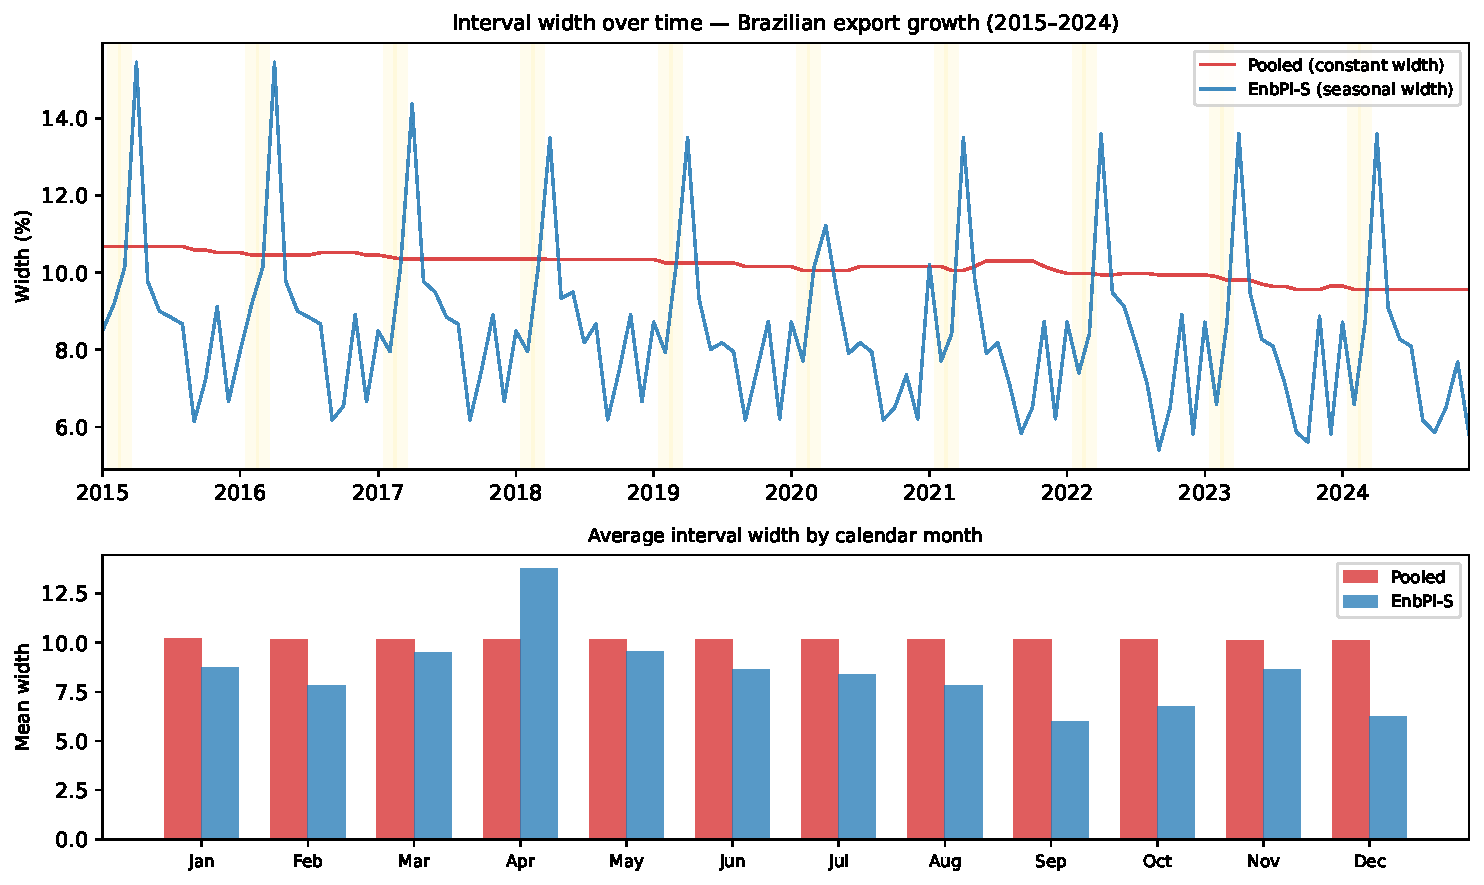
\includegraphics[width=0.95\textwidth]{figures/fig_empirical_exports_width_time}
  \caption{Interval width over time for Brazilian export growth
           (training: 1979--2014; test: 2015--2024; BCB series 1402).
           \textit{Top panel}: interval width for each month of the
           test period.  The Pooled method (red) is nearly flat at
           $\approx 10.2\%$; \texttt{EnbPI-S} (blue) peaks at
           $13.8\%$ in April (peak of the soybean harvest-export
           season) and troughs
           at $6.0\%$ in September, a ratio of $2.3\times$.
           \textit{Bottom panel}: mean interval width by calendar month.
           Gold shading marks March--May (harvest-export
           uncertainty months).}
  \label{fig:empirical_exports_width_time}
\end{figure}

\paragraph{Cross-application summary.}
Table~\ref{tab:empirical_comparison} summarises the
two applications side by side.

\begin{table}[ht]
\centering
\caption{Summary of empirical applications.
         Coverage gap $= |$empirical coverage $- 90\%|$.}
\label{tab:empirical_comparison}
\begin{tabular}{l cc cc cc}
\toprule
 & \multicolumn{2}{c}{$T_s$} &
   \multicolumn{2}{c}{Coverage gap} &
   \multicolumn{2}{c}{Width ratio} \\
\cmidrule(lr){2-3}\cmidrule(lr){4-5}\cmidrule(lr){6-7}
Application & Train & Test &
  Pooled & EnbPI-S & Pooled & EnbPI-S \\
\midrule
IPCA food (Sec.~\ref{sec:empirical:food})
  & 20 & 10 & 4.2\% & 10.8\% & 1.01 & 1.78 \\
Export growth (Sec.~\ref{sec:empirical:exports})
  & 35 & 10 & 3.3\% & 3.3\% & 1.01 & 2.30 \\
\bottomrule
\multicolumn{7}{l}{\footnotesize Width ratio = (max season width) /
  (min season width) for each method.}\\
\end{tabular}
\end{table}

The pattern across applications is consistent with
the simulation findings.
As $T_s$ increases from 20 to 35, \texttt{EnbPI-S}'s
coverage gap falls from $10.8\%$ to $3.3\%$ (a reduction of
more than two-thirds), matching Experiment E2's qualitative
prediction.
In both applications the pooled method applies a
nearly constant interval width, while \texttt{EnbPI-S}
correctly identifies and adapts to the seasonal
structure of forecast uncertainty, a conclusion
that is robust to the choice of economic series.
